% AER-Article.tex for AEA last revised 22 June 2011
\documentclass[WP]{AEA}

% The mathtime package uses a Times font instead of Computer Modern.
% Uncomment the line below if you wish to use the mathtime package:
%\usepackage[cmbold]{mathtime}
% Note that miktex, by default, configures the mathtime package to use commercial fonts
% which you may not have. If you would like to use mathtime but you are seeing error
% messages about missing fonts (mtex.pfb, mtsy.pfb, or rmtmi.pfb) then please see
% the technical support document at http://www.aeaweb.org/templates/technical_support.pdf
% for instructions on fixing this problem.

% Note: you may use either harvard or natbib (but not both) to provide a wider
% variety of citation commands than latex supports natively. See below.

% Uncomment the next line to use the natbib package with bibtex 
\usepackage{natbib}
\usepackage{hyperref}
% Uncomment the next line to use the harvard package with bibtex
%\usepackage[abbr]{harvard}

\usepackage{ amssymb }

\usepackage{amsmath}

%for \resizebox
\usepackage{graphicx}



% This command determines the leading (vertical space between lines) in draft mode
% with 1.5 corresponding to "double" spacing.
\draftSpacing{1.5}

\newtheorem{thm}{Theorm}
\newtheorem{prop}{Proposition}
\newtheorem{lemma}{Lemma}
\newtheorem{deff}{Definition}
\newtheorem{conj}{Conjecture}

\begin{document}

\title{A Theory Paper on Rank List Length}
\shortTitle{List Length}
\author{Tyler Hoppenfeld}
\date{\today}
\pubMonth{Month}
\pubYear{Year}
\pubVolume{Vol}
\pubIssue{Issue}
\JEL{}
\Keywords{}

%\begin{abstract}

\maketitle


\section{Introduction}

Centralized matching markets  encompass only a small fraction of the labor market, however the study of centralized matching markets  sheds light on the broader matching of employees to jobs. There are also a variety of markets, including academic job markets and some entry-level job markets for new college graduates, that are decentralized and sometimes chaotic despite having synchronized start dates for a large number of applicants to very similar jobs. A better understanding of the strengths and limits of centralized markets could help us understand what inefficiencies exist in these markets, whether more efficient solutions are possible, and possibly allow for the design of more efficient markets. 

Theory tells us that there is no matching mechanism that reliably produces a stable outcome wherein both sides have the incentive to report their preferences accurately \citep{Roth1985}, however in practice many matching markets persist with both sides (apparently) reporting their preferences honestly  \citep{Roth1991}. This result can be explained by the fact that in many of these markets the set of stable matchings is actually quite small, and under some realistic assumptions only agents with multiple potential stable matches have an incentive to lie about their preferences.  For example, in the National Resident Matching Program (NRMP) matching of recently graduated physicians to resident positions, all but approximately 10 of 20,000 participants have a unique partner in the set of all stable matchings \citep{Roth1999a}, and so in all but a very small number of cases any misrepresentation of preferences would lead to an identical or less-preferred outcome for the agent misrepresenting their preferences. 


Roth and Peranson posit that the small set of stable matchings (SSM) of these markets is driven by the correlated nature of preferences, and by the fact that for highly correlated preferences, the SSM is very small.  In a parallel argument, they note that finite preference lists, as is the case with the NRMP, lead to a very small SSM as well.  They use simulation to demonstrate these results, and (\cite{Immorlica2005} and then \cite{Kojima2009} build on this with the theoretical result that as the number of market participants grows, the SSM becomes arbitrarily small as a fraction of market size. This theoretical work takes short preference lists to be a feature of preferences rather than a feature of the market mechanism, and uses a highly restrictive preference structure to accomplish that. 
The primary restriction on preferences that this paper relaxes is on the existence of broadly acceptable `elite' institutions. In prior literature with $n$ residency programs and preference lists of length $k$,  at least $n-k$ institutions are unacceptable to nearly all applicants as $n$ grows without bound.  

In this paper I examine short rank lists in a setting that allows for more realistic preference formation. I construct preferences where all participants on each side in a matching market broadly share preferences over their potential matches, requiring short rank-lists does not introduce strategic behavior, and the fraction of agents with multiple stable matches has a positive limit as the market becomes infinitely large.

Additionally, I introduce an algorithm to partition the market into subsets that have limited interdependence, and prove several useful properties of these partitions.

\section{Model}
\subsection{Preliminary Definitions}

Let there be $D$ doctors and $H$ hospitals, each of which might hire at most one doctor. Doctors and hospitals together form the universe of participants $U = D \cup H$.  Each doctor $d$ has a strict preference relation over the set of hospitals he could be matched with and being unmatched, which we denote as being matched with oneself. Therefore we say that the doctor has preferences $\succ_{d}$ over the set $H \cup \{d\}$. Each hospital $h$ likewise has preferences $\succ_h$ over $D \cup \{h\}$. 

A matching $\phi$ is a mapping from $U$ onto itself such that 
\begin{itemize}
	\item for every $d$, $|\phi(d)| = 1$, $\phi(d) \in H \cup \{d\} $ and for every  $h$, $|\phi(h)| = 1$, $\phi(h) \in D \cup \{h\}$
	\item $\phi(d) = h$ iff $\phi(h) = d$.  That is, a matching is simply a one-to-one assignment of doctors to hospitals with the possibility of being unmatched. We also denote the set of all participants not matched to themselves in $\phi$ as $\{\phi\}$.
\end{itemize}
We say a matching $\phi$ is blocked by a pair $\{d,h\}$ if $h \succ_d \phi(h)$ and $d \succ_h \phi(h)$. It is individually rational if $\forall a \in U ,\phi(a) \succeq a$. A matching is stable if it is individually rational and not blocked.

\subsection{Market Participants}

The market consists of $n$ doctors  indexed $\{ d_1, d_2, ... ,d_n\}$ and  $n$ hospitals  indexed $\{ h_1, h_2, ... ,h_n\}$
	
Each doctor forms their preference list by first ranking all hospitals according to their index number, so $h_1$ is the doctor's favorite and $h_n$ their least favorite (the doctor's least favorite option is to be unmatched).  
With probability $\varepsilon$ doctor $d_1$ transposes the rankings of $h_{1}$ and $h_2$ and with probability $1-\varepsilon$ their rank list is unchanged.  For each $i  \in [1, n-1]$, with probability $\varepsilon$ doctor $d_i$ transposes the rankings of $h_{i-1}$ and $h_i$, with probability $\varepsilon$ they transposes the rankings of $h_{i+1}$ and $h_i$, and with probability $1-2\varepsilon$ their rank list is unchanged. With probability $\varepsilon$ doctor $d_n$ transposes the rankings of $h_{n-1}$ and $h_n$ and with probability $1-\varepsilon$ their rank list is unchanged.
The hospitals form their preferences in the same way.

In this way, we arrive at a preference structure where agents all broadly agree on which matches are desirable, but have idiosyncratic preference variation.
	


	
\section{Analysis}

To analyze this market I develop a method to partition the market into smaller segments that can be analyzed independently.


\subsection{An Algorithm to Partition the Market} \label{subsect:partition}

To begin, call $U_0 = D \cup H$, define $p_1(c)$ is doctor $d$'s first choice among $U_0$, and likewise for hospitals.

Next choose $d$, the doctor in $U_0$ with the lowest index number, and select $h = p_1(d)$, $d' = p_1(h)$, and so on, until a cycle is found. Call the members of that cycle $C^*$.  The algorithm proceeds as follows: 


\begin{enumerate}
	\item define the correspondence $R$ from $U_0$ to the power set $\mathcal{P}(U_0)$ such that $\forall a \in U_0, R(a) = \emptyset$
	\item for each $a \in C^*$, replace $R(a)$ =  $R(a) \cup \{p_1(a)\}$
	\item  \label{seg_alg:comp} for each $a \in U_0$, and $b \in U_0$, if $ b \in R(a)$ replace $R(b) = \{a\} \cup R(b)$
	\item  \label{seg_alg:ext} for each $a \in U_0$ such that $R(a) \neq \emptyset$, call  $c$ their least preferred member of $R(a)$. Now, for each $\delta \in U_0 | \delta \succ_a c$, replace $R(a) = R(a) \cup \delta$ 
	\item if $R$ has been altered in step \ref*{seg_alg:comp} or \ref*{seg_alg:ext}, return to step \ref*{seg_alg:comp}, otherwise proceed
	\item call $C_0$ the set of all agents for whom $R(a) \neq \emptyset$
	\item Perform doctor-proposing deferred acceptance on $C_0$, and call the result $\phi_{d0}$
\end{enumerate}

To find the next partition, call $U_1 = U_0 \setminus \{\phi_{d0}\}$, and repeat the entire process to find $C_1$ and $\phi_{d1}$

The algorithm ends when $\{\phi_{di}\} = \emptyset$ or $C_i= \emptyset$.  We call $\phi_d = \{\phi_{d0}, \phi_{d1}, ...\}$.

\begin{lemma}
	$ U \setminus \{\phi_{d}\} \subseteq D$ or $ U \setminus \{\phi_{d}\} \subseteq H$ 
\end{lemma}

\begin{proof}
	First note that If $\{\phi_{di}\} = \emptyset$, $C_i \subseteq H$ or $C_i \subseteq D$ because all doctors are acceptable to all hospitals, and vice-versa. This also implies that if $C_i \subseteq H$ or $C_i \subseteq H$, all unmatched agents are from the same side of the market.  Thus the process ends only when all agents are matched, or when the only unmatched agents are from the same side.
\end{proof}

\begin{lemma}
	$\{\phi_{di}\}=\{\phi_{hi}\}$
\end{lemma}
\begin{proof}
	This is an application of the rural hospitals theorem, which says that the set of unmatched agents is the same in all stable matchings \cite{Roth1986}.
\end{proof}

\begin{prop} \label{prop:equiv}
	$\phi_d $ is identical to the doctor proposing deferred acceptance matching $\Phi_d $
\end{prop}
\begin{proof}
	
 To show this, we will run deferred acceptance in a particular order to find $\Phi_d$ with a useful intermediate stage
 \begin{enumerate}
 	\item Call $D_0=D\cap C_0$, $H_0 = H \cap C_0$,$H_1 = H \cap C_1$, etc
 	\item Call $p(d)$ $d$'s favorite hospital in $H$ who has not yet rejected them, or the doctor themself if they have been rejected by all acceptable hospitals
 	\item \label{step:restricted_prop} Next, each $d \in D_0$ proposes to $p(d)$ only if $p(d) \in C_0$
 	\item \label{step:reject} Hospitals hold and reject offers as in standard deferred acceptance
 	\item repeat steps \ref{step:restricted_prop} and \ref{step:reject} until no more proposals are made
 	\item Call this intermediate matching $\Phi_{d0}$, and note that $\Phi_{d0} = \phi_{d0}$
 	\item \label{step:restricted_prop_ext} Next each unmatched doctor $d \in D_1$ proposes to $p(d)$ if $p(d) \in \{\Phi_{d0}\} \cup C_1$
 	\item \label{step:reject_ext} Hospitals hold and reject offers as in standard deferred acceptance 	
 	\item repeat steps \ref{step:restricted_prop_ext} and \ref{step:reject_ext} until no more proposals are made. 
 	\item note that no hospital in $\{\Phi_{d0}\}$ will reject its current match in favor of a doctor $d\notin C_0$, so no doctor in $\{\Phi_{d0}\}$ will be rejected, and so no match in $\{\Phi_{d0}\}$  will be disrupted
 	\item Call the current match  $\Phi_{d\{0,1\}}= \phi_{d0} \cup \phi_{d1}$
 	\item return to step \ref{step:restricted_prop_ext} for the sets $D_2, D_3, ...$ for each partition.
 	\item If there are any remaining unmatched doctors, allow them to propose to each hospital who has not yet rejected them. They will be rejected by all hospital without ever being held, even temporarily.  
 	\item Thus we have reached the end of deferred acceptance, and shown that $\Phi_{d\{0,1,2,...\}}= \phi_{d} =\Phi_{d}$
  \end{enumerate}
\end{proof}






\subsection{Analyzing the model} \label{subsect:partition}

We begin by partitioning the market as in subsection \ref{subsect:partition} . 

There are 16 possible preference relation sets for the participants $\{d_1,d_2,h_1,h_2\}$, enumerated in the appendix. These relation sets can be grouped into four groups, A-D.

Type A: This is the simplest case, in which $d_1$ and $d_2$ both prefer $h_1$ to $h_2$, and both $h_1$ and $h_2$ prefer $d_1$ to $d_2$.  In this case $C_0 =\{d_1,h_1\}$ and $\{\phi_0\}=\{d_1,h_1\}$. 
Conditional on $\{d_1,d_2,h_1,h_2\}$ having Type A preferences, $\{d_2,d_3,h_2,h_3\}$ are drawn from the same distribution as $\{d_1,d_2,h_1,h_2\}$.  

Type B: In eleven cases preferences are such that $ \{\phi_0\} \cup \{\phi_1\}=\{d_1,d_2,h_1,h_2\} $.
Conditional on $\{d_1,d_2,h_1,h_2\}$ having Type B preferences, $\{d_3,d_4,h_3,h_4\}$ are drawn from the same distribution as $\{d_1,d_2,h_1,h_2\}$.  

Type C: In two cases  $\{\phi_1\}=C_0 = \{d_1,d_2,h_1,h_2\}$, and in these two cases multiple stable matching are possible.  Conditional on $\{d_1,d_2,h_1,h_2\}$ having Type C preferences, $\{d_3,d_4,h_3,h_4\}$ are drawn from the same distribution as $\{d_1,d_2,h_1,h_2\}$.  

Type D: In two cases $\{\phi_0\}= C_0=\{d_1,h_1\}$, but these cases are distinguished because conditional on $\{d_1,d_2,h_1,h_2\}$ having Type D preferences, $\{d_3,d_4,h_3,h_4\}$ are drawn from  a restricted distribution.

As the partition algorithm progresses through the rank lists it transitions through these cases as a Markov chain with the transition matrix:


 \begin{equation*}
 	\resizebox{\textwidth}{!}{
$	\Pi = 
	\left[
		\begin{matrix}
			\left(1 - \epsilon\right)^{4} & \epsilon^{4} + 4 \epsilon^{2} \left(1 - \epsilon\right)^{2} + 6 \epsilon \left(1 - \epsilon\right)^{3} & 2 \epsilon^{2} \left(1 - \epsilon\right)^{2} & 2 \epsilon \left(1 - \epsilon\right)^{3}\\\left(1 - \epsilon\right)^{4} & \epsilon^{4} + 4 \epsilon^{2} \left(1 - \epsilon\right)^{2} + 6 \epsilon \left(1 - \epsilon\right)^{3} & 2 \epsilon^{2} \left(1 - \epsilon\right)^{2} & 2 \epsilon \left(1 - \epsilon\right)^{3}\\\left(1 - \epsilon\right)^{4} & \epsilon^{4} + 4 \epsilon^{2} \left(1 - \epsilon\right)^{2} + 6 \epsilon \left(1 - \epsilon\right)^{3} & 2 \epsilon^{2} \left(1 - \epsilon\right)^{2} & 2 \epsilon \left(1 - \epsilon\right)^{3}\\\frac{\left(1 - \epsilon\right)^{4}}{3 \epsilon^{2} \left(1 - \epsilon\right)^{2} + 4 \epsilon \left(1 - \epsilon\right)^{3} + \left(1 - \epsilon\right)^{4}} & \frac{2 \epsilon^{2} \left(1 - \epsilon\right)^{2} + 2 \epsilon \left(1 - \epsilon\right)^{3}}{3 \epsilon^{2} \left(1 - \epsilon\right)^{2} + 4 \epsilon \left(1 - \epsilon\right)^{3} + \left(1 - \epsilon\right)^{4}} & \frac{\epsilon^{2} \left(1 - \epsilon\right)^{2}}{3 \epsilon^{2} \left(1 - \epsilon\right)^{2} + 4 \epsilon \left(1 - \epsilon\right)^{3} + \left(1 - \epsilon\right)^{4}} & \frac{2 \epsilon \left(1 - \epsilon\right)^{3}}{3 \epsilon^{2} \left(1 - \epsilon\right)^{2} + 4 \epsilon \left(1 - \epsilon\right)^{3} + \left(1 - \epsilon\right)^{4}}
		\end{matrix}
	\right] 
	$
}
\end{equation*}

and the stationary distribution:
 \begin{equation*}
	\resizebox{\textwidth}{!}{
		$	
		\left[\begin{matrix}\frac{14 \epsilon^{5} - 17 \epsilon^{4} + 8 \epsilon^{3} - 10 \epsilon^{2} + 6 \epsilon - 1}{4 \epsilon^{5} - 10 \epsilon^{4} + 6 \epsilon^{3} - 2 \epsilon - 1} & \frac{2 \epsilon^{6} - 16 \epsilon^{5} + 17 \epsilon^{4} - 10 \epsilon^{3} + 10 \epsilon^{2} - 6 \epsilon}{4 \epsilon^{5} - 10 \epsilon^{4} + 6 \epsilon^{3} - 2 \epsilon - 1} & \frac{- 2 \epsilon^{6} + 2 \epsilon^{5} + 2 \epsilon^{3} - 2 \epsilon^{2}}{4 \epsilon^{5} - 10 \epsilon^{4} + 6 \epsilon^{3} - 2 \epsilon - 1} & \frac{4 \epsilon^{5} - 10 \epsilon^{4} + 6 \epsilon^{3} + 2 \epsilon^{2} - 2 \epsilon}{4 \epsilon^{5} - 10 \epsilon^{4} + 6 \epsilon^{3} - 2 \epsilon - 1}\end{matrix}\right] 
		$
	}
\end{equation*}




Now I turn my attention to type C. Consider the sub-case in which $h_2\succ_{d_1} h_1$ and $d_2\succ_{h_2} d_2$.  With probability $p=\epsilon$ $h_3\succ_{d_2} h_2$, in which case $C_0 =\{d_1,h_1,d_2,h_2, h_3\}$, and $\phi_0=\{(d_1:h_2),(d_2:h_1)\}$ is the only stable matching.  With probability $p=1-\epsilon$ $h_2\succ_{d_2} h_3$, in which case $C_0 =\{d_1,h_1,d_2,h_2\}$, and $\phi_{d0}=\{(d_1:h_2),(d_2:h_1)\}$ and $\phi_{h0}=\{(d_1:h_1),(d_2:h_2)\}$ are both stable matchings.  Likewise, in the subcase where  $h_2\succ_{d_2} h_1$ and $d_2\succ_{h_1} d_2$, $d_3\succ_{h_2} d_2$ with  probability $p=1- \epsilon$, in which case  $C_0 =\{d_1,h_1,d_2,h_2\}$, and $\phi_{d0}=\{(d_1:h_2),(d_2:h_1)\}$ and $\phi_{h0}=\{(d_1:h_1),(d_2:h_2)\}$ are both stable matchings.

Now we calculate the fraction of agents with more than one stable matching.  

First, note that, on average, each Markov chain step advances through the preference lists by the distance:

\begin{equation*}
		\resizebox{\textwidth}{!}{
		$	
			\frac{2 \left(- 2 \epsilon^{6} + 2 \epsilon^{5} + 2 \epsilon^{3} - 2 \epsilon^{2}\right)}{4 \epsilon^{5} - 10 \epsilon^{4} + 6 \epsilon^{3} - 2 \epsilon - 1} + \frac{4 \epsilon^{5} - 10 \epsilon^{4} + 6 \epsilon^{3} + 2 \epsilon^{2} - 2 \epsilon}{4 \epsilon^{5} - 10 \epsilon^{4} + 6 \epsilon^{3} - 2 \epsilon - 1} + \frac{14 \epsilon^{5} - 17 \epsilon^{4} + 8 \epsilon^{3} - 10 \epsilon^{2} + 6 \epsilon - 1}{4 \epsilon^{5} - 10 \epsilon^{4} + 6 \epsilon^{3} - 2 \epsilon - 1} + \frac{2 \left(2 \epsilon^{6} - 16 \epsilon^{5} + 17 \epsilon^{4} - 10 \epsilon^{3} + 10 \epsilon^{2} - 6 \epsilon\right)}{4 \epsilon^{5} - 10 \epsilon^{4} + 6 \epsilon^{3} - 2 \epsilon - 1}
		$
	}
\end{equation*}

and so the fraction of agents who have multiple stable equilibria:

\begin{equation*}
	\resizebox{\textwidth}{!}{
	$
			\frac{2 \left(1 - \epsilon\right) \left(- 2 \epsilon^{6} + 2 \epsilon^{5} + 2 \epsilon^{3} - 2 \epsilon^{2}\right)}{\left(\frac{2 \left(- 2 \epsilon^{6} + 2 \epsilon^{5} + 2 \epsilon^{3} - 2 \epsilon^{2}\right)}{4 \epsilon^{5} - 10 \epsilon^{4} + 6 \epsilon^{3} - 2 \epsilon - 1} + \frac{4 \epsilon^{5} - 10 \epsilon^{4} + 6 \epsilon^{3} + 2 \epsilon^{2} - 2 \epsilon}{4 \epsilon^{5} - 10 \epsilon^{4} + 6 \epsilon^{3} - 2 \epsilon - 1} + \frac{14 \epsilon^{5} - 17 \epsilon^{4} + 8 \epsilon^{3} - 10 \epsilon^{2} + 6 \epsilon - 1}{4 \epsilon^{5} - 10 \epsilon^{4} + 6 \epsilon^{3} - 2 \epsilon - 1} + \frac{2 \left(2 \epsilon^{6} - 16 \epsilon^{5} + 17 \epsilon^{4} - 10 \epsilon^{3} + 10 \epsilon^{2} - 6 \epsilon\right)}{4 \epsilon^{5} - 10 \epsilon^{4} + 6 \epsilon^{3} - 2 \epsilon - 1}\right) \left(4 \epsilon^{5} - 10 \epsilon^{4} + 6 \epsilon^{3} - 2 \epsilon - 1\right)}
	$
}
\end{equation*}

Finally I plot this expression as a function of $\epsilon$ in figure \ref{fig:multi_match}, showing that in the large market limit there are multiple stable matches for many agents over a wide range of $\epsilon$ values.

\begin{figure}[p]{Fraction of Agents With Multiple Stable Matchings}
	\resizebox{\textwidth}{!}{
		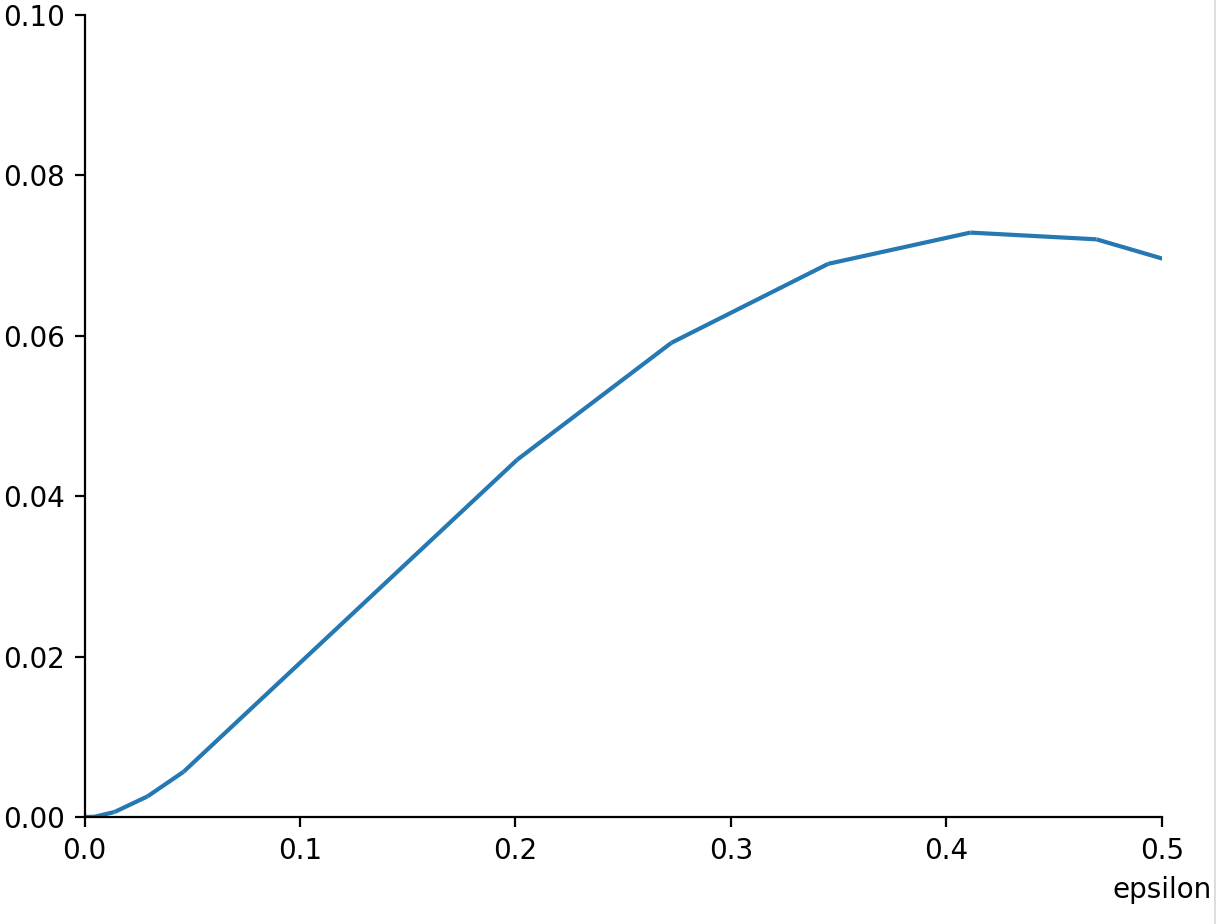
\includegraphics{mult_frac_ep}	
	}
	\caption{The fraction of agents with more than one stable match as a function of $\epsilon$}
	\label{fig:multi_match}
\end{figure}

\subsection{Rank List Length}

\begin{prop}
	Agents are indiferent between submitting a three-entry rank list and their complete preferences.
\end{prop}

\begin{proof}
	As we partition the market as in subsection \ref{subsect:partition}, there is never a case where two agents in the same partition have index numbers that differ by more than one. Therefore, the partitions and resultant matching are the same if each person submits a 3-member rank list consisting of only agents they might share a partition with.
\end{proof}





\bibliographystyle{aea}
\bibliography{../../library}

% The appendix command is issued once, prior to all appendices, if any.
\appendix



\section{ Appendix}

\subsection{Deferred Acceptance}
The deferred acceptance mechanism is a mainstay of this paper. In the doctor-proposing version of this mechanism, the algorithm iteritavely selects a doctor $d$ who proposes to their most preferred hospital that has not yet rejected them, unless the doctor has been rejected by all hospitals who they prefer to being unmatched.  If the hospital prefers the proposing doctor to the current tenative assignment, the hospital holds the doctor's proposal and rejects their current assignment (if one exists). Otherwise, the hospital rejects $d$.  This process repeats until all doctors are either tentatively matched or have run out of proposals to make, and arrives at a stable matching that is weakly preferred by all doctors to any other stable matching.  We call this the doctor-optimal stable match, because it is weakly preferred by all doctors to any other stable match.  A parallel result exists for the hospital-proposing algorithm.


\subsection{Permutations of preferences for $\{d_1,d_2,h_1,h_2\}$}
I denote preferences with a four-bit binary number, in which a zero in the first position indicates that $h_1\succ_{d_1} h_2$ while a one in the first position indicates that $h_1\prec_{d_1} h_2$. Likewise the second through fourth positions indicate the preferences of $d_2, ,h_1$,and $h_2$.
\\
Type A

$(0,0,0,0)$: $C_0 =\{d_1,h_1\}, \{\phi_0\}=\{d_1,h_1\}$.  Preferences for $\{d_2,d_3,h_2,h_3\}$ are unrestricted.
\\

Type B

$(0,0,1,0)$: $C_0 =\{d_2,h_1\}, \{\phi_0\}=\{d_2,h_1\}, C_1 =\{d_1,h_2\}, \{\phi_1\}=\{d_1,h_2\}$.  Preferences for $\{d_3,d_4,h_3,h_4\}$ are unrestricted.


$(0,0,1,1)$: $C_0 =\{d_2,h_1\}, \{\phi_0\}=\{d_2,h_1\}, C_1 =\{d_1,h_2\}, \{\phi_1\}=\{d_1,h_2\}$.  Preferences for $\{d_3,d_4,h_3,h_4\}$ are unrestricted.


$(0,1,0,1)$: $C_0 =\{d_1,h_1\}, \{\phi_0\}=\{d_1,h_1\}, C_1 =\{d_2,h_2\}, \{\phi_1\}=\{d_2,h_2\}$.  Preferences for $\{d_3,d_4,h_3,h_4\}$ are unrestricted.


$(0,1,1,1)$: $C_0 =\{d_2,h_2\}, \{\phi_0\}=\{d_2,h_2\}, C_1 =\{d_1,h_1\}, \{\phi_1\}=\{d_1,h_1\}$.  Preferences for $\{d_3,d_4,h_3,h_4\}$ are unrestricted.


$(1,0,0,0)$: $C_0 =\{d_1,h_2\}, \{\phi_0\}=\{d_1,h_2\}, C_1 =\{d_2,h_1\}, \{\phi_1\}=\{d_2,h_1\}$.  Preferences for $\{d_3,d_4,h_3,h_4\}$ are unrestricted.


$(1,0,1,0)$: $C_0 =\{d_1,h_2\}, \{\phi_0\}=\{d_1,h_2\}, C_1 =\{d_2,h_1\}, \{\phi_1\}=\{d_2,h_1\}$.  Preferences for $\{d_3,d_4,h_3,h_4\}$ are unrestricted.


$(1,0,1,1)$: $C_0 =\{d_2,h_1\}, \{\phi_0\}=\{d_2,h_1\}, C_1 =\{d_1,h_2\}, \{\phi_1\}=\{d_1,h_2\}$.  Preferences for $\{d_3,d_4,h_3,h_4\}$ are unrestricted.



$(1,1,0,0)$:  $C_0 =\{d_1,h_2\}, \{\phi_0\}=\{d_1,h_2\}, C_1 =\{d_2,h_1\}, \{\phi_1\}=\{d_2,h_1\}$.  Preferences for $\{d_3,d_4,h_3,h_4\}$ are unrestricted.


$(1,1,0,1)$:  $C_0 =\{d_2,h_2\}, \{\phi_0\}=\{d_2,h_2\}, C_1 =\{d_1,h_1\}, \{\phi_1\}=\{d_1,h_1\}$.  Preferences for $\{d_3,d_4,h_3,h_4\}$ are unrestricted.



$(1,1,1,0)$:  $C_0 =\{d_1,h_2\}, \{\phi_0\}=\{d_1,h_2\}, C_1 =\{d_2,h_1\}, \{\phi_1\}=\{d_2,h_1\}$.  Preferences for $\{d_3,d_4,h_3,h_4\}$ are unrestricted.



$(1,1,1,1)$:  $C_0 =\{d_2,h_2\}, \{\phi_0\}=\{d_2,h_2\}, C_1 =\{d_1,h_1\}, \{\phi_1\}=\{d_1,h_1\}$.  Preferences for $\{d_3,d_4,h_3,h_4\}$ are unrestricted.
\\

Type C

$(1,0,0,1)$:  $C_0 =\{d_1,h_1,d_2,h_2\}$ or $C_0 =\{d_1,h_1,d_2,h_2, h_3\}$ if $h_3\succ_{d_2} h_2$, $\{\phi_0\}=\{d_1,d_1,h_2,h_2\}$.  Preferences for $\{d_3,d_4,h_3,h_4\}$ are unrestricted. 

$(0,1,1,0)$:  $C_0 =\{d_1,h_1,d_2,h_2\}$ or $C_0 =\{d_1,h_1,d_2,h_2, d_3\}$ if $d_3\succ_{h_2} d_2$, $\{\phi_0\}=\{d_1,h_1,d_2,h_2\}$.  Preferences for $\{d_3,d_4,h_3,h_4\}$ are unrestricted. 
\\


Type D

$(0,0,0,1)$:  $C_0 =\{d_1,h_1\}, \{\phi_0\}=\{d_1,h_1\}$.  Preferences for $\{d_2,d_3,h_2,h_3\}$ fit the pattern $(\cdot,\cdot,0,\cdot)$.


$(0,1,0,0)$:  $C_0 =\{d_1,h_1\}, \{\phi_0\}=\{d_1,h_1\}$.  Preferences for $\{d_2,d_3,h_2,h_3\}$ fit the pattern $(0,\cdot,\cdot,\cdot)$.



\end{document}

